\chapter{Semantic Web Architecture}

Semantic web uses URI to identify an existing name or resource, RDF/RDFS and OWL to store new information, and SPARQL to query from the knowledge base. The semantic web stack is already given earlier in Section \ref{subsec:semanticwebstack}. More details are introduced in this chapter.

\section{Uniform Resource Identifier (URI)}

Humans uses symbol and concept to help interpret things and link to objects in real life. This is demonstrated by semiotic triangle as shown in Fig. \ref{fig:semiotictriangle}. The interpretation of ``apple'' is used as an example.

\begin{figure}[htbp]
	\centering
	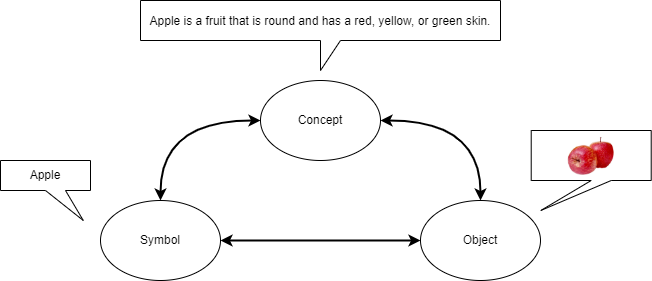
\includegraphics[width=0.8\textwidth]{./chapters/ch-semanticwebarchitecture/figures/semiotic_triangle.png}
	\caption{Semiotic triangle.}
	\label{fig:semiotictriangle}
\end{figure} 



\section{Resource Description Framework (RDF)}

\section{RDF Schema}

\section{SPARQL Protocol and RDF Query Language (SPARQL)}

\section{Web Ontology Language (OWL)}
